

\section{Building blocks}
\label{building-blocks}

The ScopeSim framework has been designed to maintain strict boundaries between the simulation code, the optical model data, and the user input.
%As with real systems, the astronomical objects and the light they emit exist regardless of the telescope or astronomer.
%The telescope and instruments also exist independently of the astronomer.
%Only when an astronomer uses a telescope to observe a celestial object are the three connected.
A similar philosophy has been applied to the development of the ScopeSim framework.

The ScopeSim framework consists of three main packages:
\begin{itemize}
\item \lstinline{ScopeSim}: the core simulation engine,

\item \lstinline{ScopeSim_templates}: a library of functions for generating descriptions of on-sky objects,

\item \lstinline{IRDB}: The instrument reference database containing the data and configuration files needed to generate the digital models of a range of telescope and instrument optical system.
\end{itemize}

\begin{figure}

\resizebox{\linewidth}{!}{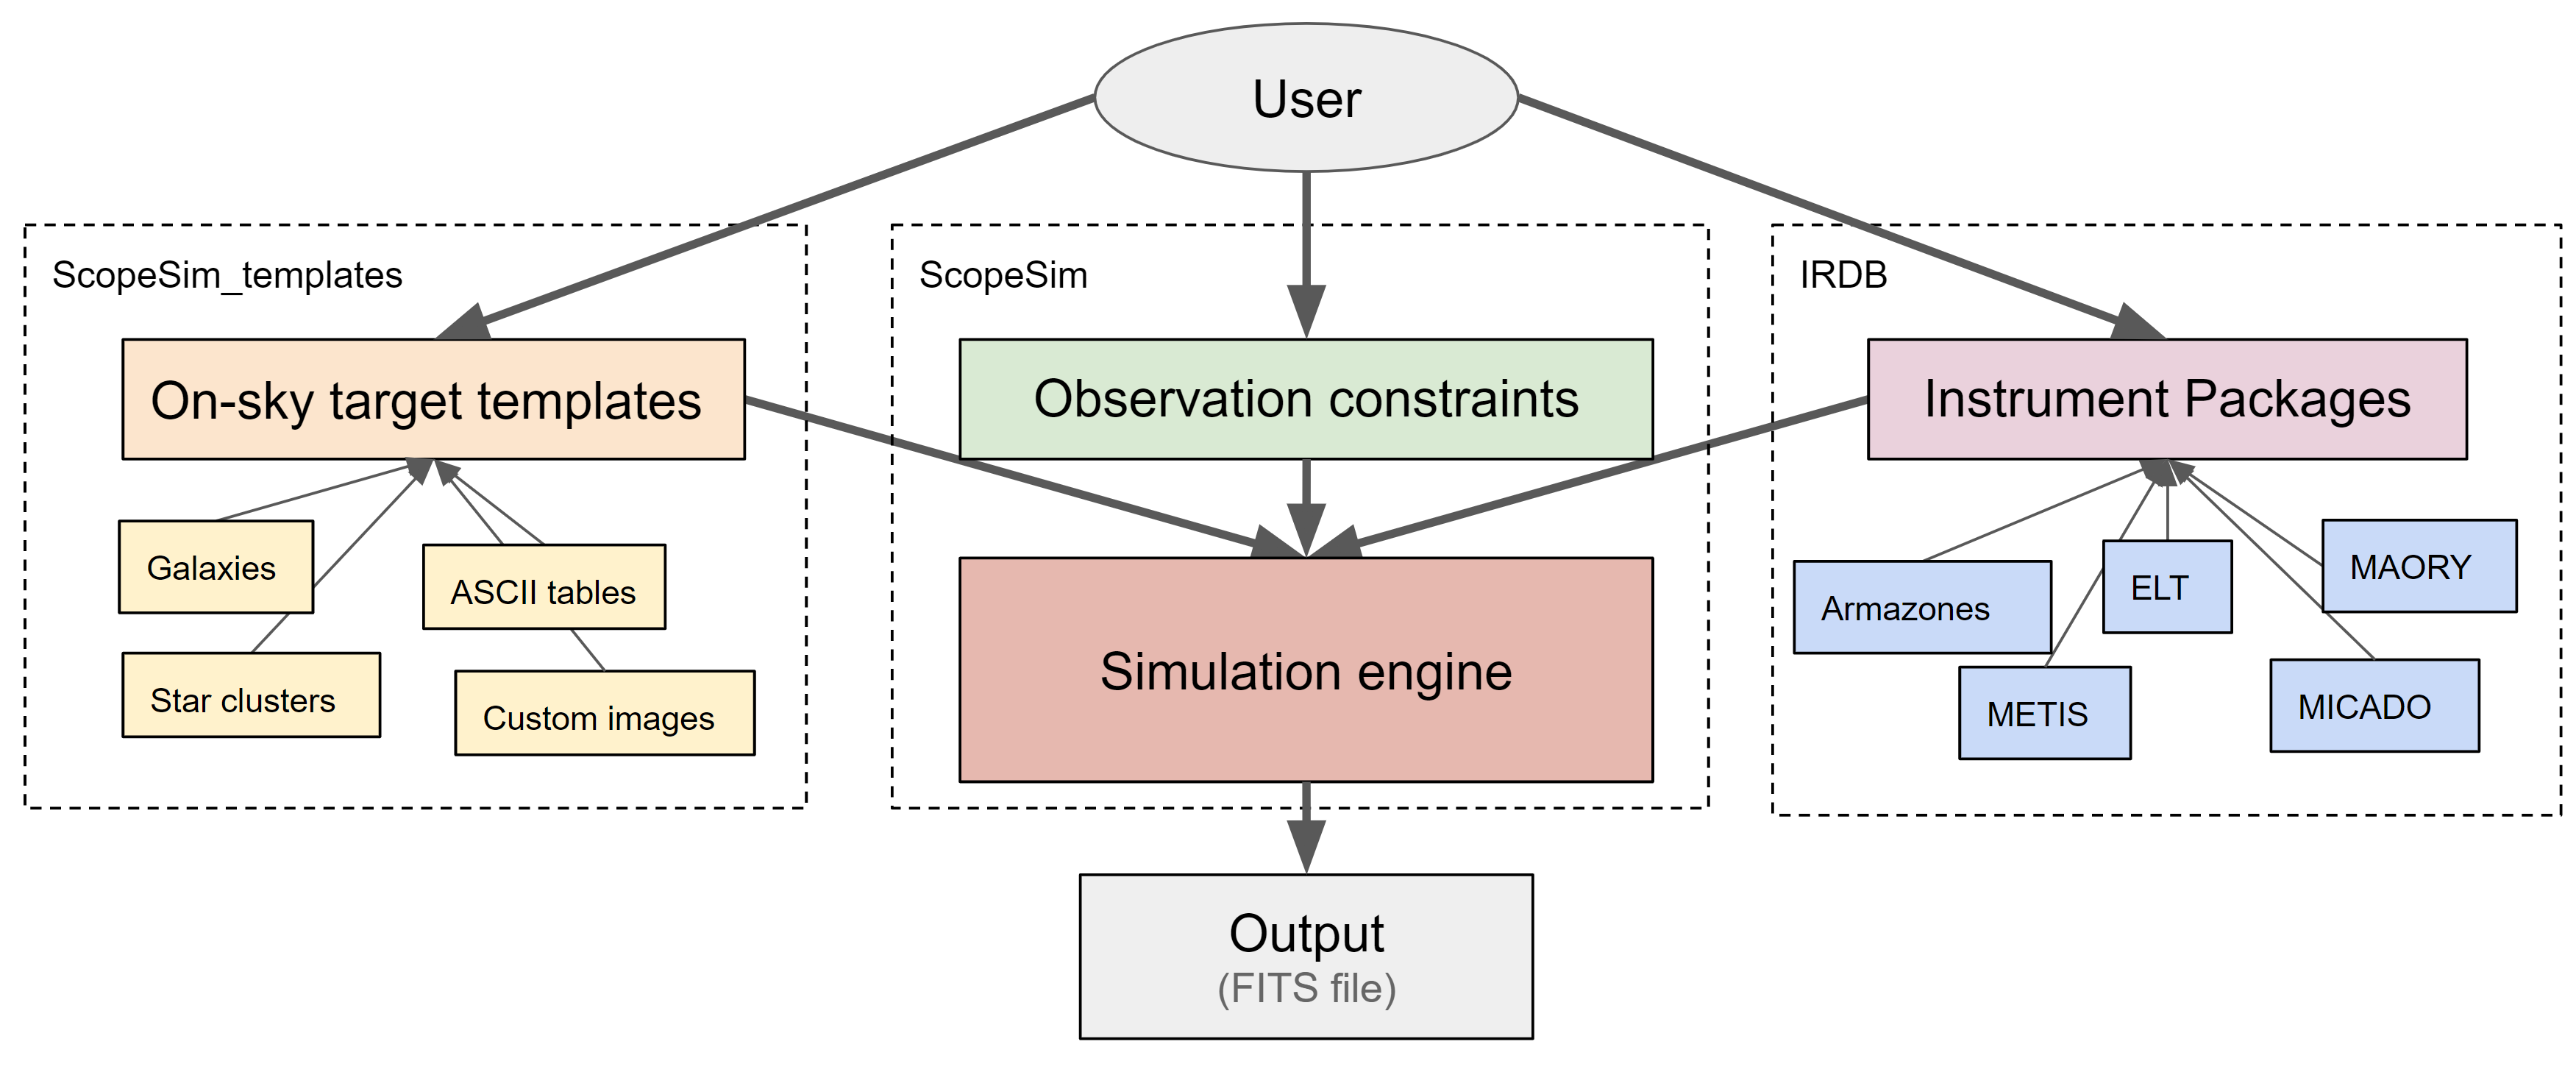
\includegraphics{Ecosystem.png}}
\caption{An illustration of the scopes of the three main packages in the ScopeSim environment.
\lstinline{ScopeSim_templates} (left) only provides the functionality to generate descriptions of on-sky objects in the format used by ScopeSim.
The instrument reference database (right) contains the data and configuration files required to generate a model of an optical system in discrete instrument packages.
The ScopeSim engine (centre) requires input from both of these packages, along with the observation constraints (e.g.~exposure time, observing mode, etc.) in order to simulate mock observation data.
The final output of a simulation is one or more FITS files containing the images or spectra of the user's  target including all expected optical aberrations associated with the optical system.}
\label{fig:framework}

\end{figure}

Figure~\ref{fig:framework} illustrates the relationship between these three packages.
Although there is a strict delineation between the scopes of each package, the interfaces between the packages allow them to interact almost seamlessly with each other.
This can be seen in the code examples from Section~\ref{examples}.
The main code pattern for simulating observations with a specific instrument is the same for all use cases:

\begin{enumerate}
\item download the required instrument packages from the instrument reference database (IRDB) using \lstinline{scopesim},

\item create a description of the astronomical object using \lstinline{scopesim_templates},

\item generate a model of the desired optical system using \lstinline{scopesim} and referencing the \lstinline{irdb} package,

\item simulate and output the observed data using \lstinline{scopesim}.
\end{enumerate}

The following subsections briefly describe each of these three packages.

\subsection{ScopeSim: the observation simulator engine}
\label{scopesim-the-observation-simulator-engine}

The ScopeSim core package, also referred to as the ScopeSim engine, contains the code necessary for running observations simulations.
The code has been written in such a way as to be completely agnostic to the instrument setup as well as agnostic towards the on-sky target.
At its heart the code transports flux from a description of the on-sky target to a detector focal plane.
During the process it applies any optical aberrations contained in the optical model to the flux description.
Section~\ref{scopesim-architecture} describes this process in more detail.
ScopeSim attempts to remove as much redundancy and inefficiency from observation simulations as possible by recognising the fact that there is little need to redo the majority of the calculations executed in high-fidelity simulations.
In other words, the ScopeSim engine does not work with ray-tracing methods or use Fourier optics, except in isolated cases.
Instead it uses the fact that the observed image is a linear combination of independent optical aberrations applied to an incoming spectro-spatial flux distribution.

This focus on removing as many redundant calculations as possible results in very quick execution times.
The images from the code examples were generated on a standard laptop in around 10~seconds.
Such speed makes ScopeSim suitable for use cases with short iteration times, such a quick look feasibility studies, e.g.~``playing'' with a science case, or advanced exposure time calculators.
At the other end of the scale, ScopeSim is also useful for generating simulated raw data needed during the development of instrument data reduction pipelines.
As the ScopeSim engine takes its cues from the instrument packages, the fidelity of simulations is limited only the number and accuracy of the Effects listed in these packages.


\subsection{ScopeSim Templates: Descriptions of on-sky targets}
\label{scopesim-templates-descriptions-of-on-sky-targets}

The \scopesimtemplates{} package provides a series of functions to help the user create a description of the on-sky targets they wish to observe in the format required by the \ScopeSim{} engine.
These helper function populate one or more instances of the \ScopeSim{} \Source{} class with the data needed to best describe the target.


\subsubsection{Format of a Source object}
\label{format-of-a-source-object}

In order to optimise memory usage the \Source{} objects split the spatial and spectral characteristics of a target.\cite{schmalzl2012}
These are held separately in two lists: fields and spectra.
A spatial field can be either a table of coordinated and flux scaling factors (e.g.~the positions of stars in cluster) or a 2D weight map (e.g.~an image of a galaxy).
Each entry in a field must reference one of the entries in the list of spectra, although there is no requirement for a one-to-one relationship between field entries and spectral list entries.
For example in the case of star cluster, all A0V stars can reference a single A0V spectrum.
\ScopeSim{} memory requirements are further reduced by taking advantage of this redundancy.

Galaxies and similar extended objects can also be adequately represented in this manner.
A galaxy generally contains populations of stars (new, old, high- or low-metallicity, etc.) and in most cases observations do not resolve individual stars.
Hence it can be assumed that if each component is represented by a unique flux weight map (i.e.~an image) then each stellar population can be represented by a single spectrum.
As an example, the \scopesimtemplates{} function \lstinline{galaxy.spiral_two_component} uses the B~filter image of the galaxy NGC\,1232L to represent the young population and the I~filter image for the old population.
Each image references a spectrum for a young or old population.

The extreme limit for this type of representation would be the case where every single pixel in an image is associated with a unique spectrum.
An example might be the turbulent motions of gas in a star forming region, although it is still arguable that even here there will still be spectrally redundant regions.
In this case the spectral and spatial components can still be split, although the result will be that each spatial field entry will consist of an image with only a single pixel and referencing the associated spectrum from the list of spectra.
Such a use case would be particularly computationally expensive.
It is therefore highly recommended in such cases to search for possible spectral redundancy before creating a \Source{} object from a spectral cube.


\subsubsection{Structure of ScopeSim templates package}
\label{structure-of-scopesim-templates-package}


Currently \ScopeSimtemplates{} splits the helper functions into categories based on the complexity of the Source object that is produced.
The \lstinline{basic} subpackage contains helper functions that are useful for quick look investigations, but which should not be used for in-depth feasibility studies.
For example the \lstinline{stars.cluster} function does not allow age or metallicity to be set.
In contrast the \lstinline{advanced} subpackage contains functions that can be useful for very specific science cases, but are not adapted for general use.

In addition to the general functions, it is possible to add helper functions for objects used by specific instruments.
The \lstinline{micado} subpackage for example contains functions that produce objects specific to the MICADO instrument at the ELT.
Community participation is most welcome to help expand the number of object template function in the \ScopeSimtemplates{} package.


\subsection{Instrument Reference Database: The optical model data}
\label{instrument-reference-database-the-optical-model-data}

\ScopeSim{} aims to be a general-purpose instrument data simulator that can be used to simulate the output of many different optical systems.
To make this goal a reality it was mandatory that the \scopesim{} engine be completely instrument agnostic.
There is however a large amount of instrument specific data that is needed to accurately model the optical aberrations inherent in any optical system.
For \ScopeSim{} this data is stored in instrument packages in a separate instrument reference database (IRDB).
Instrument packages can be created for any self-contained section of an optical train.
For example, the telescope, the atmosphere, the relay optics, and the instrument are generally assumed to be self-contained optical sections.
For small observatories like the University of Vienna's 1.5\,m telescope there is no benefit to splitting the optical elements into separate packages.
However, for large observatories like the VLT where multiple instruments can be attached to a single telescope, it makes sense to split the telescope optical system from the instrument description.
Not only does this avoid multiple versions of a single optical element (e.g.~telescope) becoming unsynchronised when one instrument package is updated and another is not, it also reduces the scope of responsibility for maintaining packages.
For example, this means that instrument consortia need only concentrate on maintaining their own instrument package, while the telescope operator is responsible for maintaining the telescope package.
It also means a telescope or relay optics package can be updated without needing (theoretically) to inform the maintainers of all instrument packages that use those subsystem.


\subsubsection{Instrument package format}
\label{instrument-package-format}

Each instrument package contains two main types of data:
\begin{enumerate}
\item A series of configuration files describing which optical aberrations should be modelled by \scopesim{}, and

\item The empirical data files needed for \scopesim{} to apply the aberrations to the incoming photon flux.
\end{enumerate}

The configuration files are written in YAML.
They contain lists of \Effect{} object descriptions as well as global properties that are common to all \Effect{} objects in the subsystem.
The \Effect{} object descriptions must call an existing \Effect{} class from the \ScopeSim{} core package.
\Effect{} objects are discussed in more detail in Section~\ref{effects-objects}.
For the \Effect{}s that rely on external empirical data, these files must also be contained in the instrument package.
The empirical data files must be either ASCII tables or FITS images/tables.
Examples of empirical data files include the filter response curves or pre-computed sets of PSF kernels.

The raw instrument data currently resides in the instrument reference database on Github.
Periodically, or when explicitly needed, the data on this repository are compiled into packages and uploaded onto the \ScopeSim{} server.
It is from here that \ScopeSim{} downloads a package when asked to do so by the user (as seen in the code examples).
Packages are downloaded using \lstinline{Astropy}, and hence are saved locally in the \lstinline{Astropy} cache.
This allows the packages to be used offline.
Updated packages can be downloaded by either clearing the \lstinline{Astropy} cache, or by forcing \scopesim{} to redownload a package via the RC parameters.
An example of this is available in the online documentation.

For readers interested in creating their own instrument packages for a local telescope or instrument, the authors recommend looking inside the \lstinline{LFOA} (Leopold Figl Observatory for Astrophysics) package on the IRDB Github page.
This contains everything needed to simulate observations with the Viennese 1.5\,m telescope.



\subsection{Support Packages}
\label{support-packages}

In addition to the core package, there are several support packages:

\begin{itemize}
\item \lstinline{AnisoCADO}: simulates SCAO PSFs for the ELT

\item \lstinline{SkyCalc_ipy}: queries the ESO skycalc service for atmospheric spectral curves

\item \lstinline{SpeXtra}: provides easy access to many well-known spectral libraries

\item \lstinline{Pyckles}: a light-weight wrapper for the Pickles (1998) and Brown (2010) catalogues.
\end{itemize}

These package are not direct dependencies of \ScopeSim{}, but do help provide additional functionality to the simulation engine.
Table~\ref{tbl-list-of-packages} contains a list of the relevant links to both documentation and code-bases for these packages.

\begin{table}
\caption{Links to the open source documentation and code bases}
\label{tbl-list-of-packages}
\begin{tabularx}{\linewidth}{|l|X|X|}
\hline

Package
 &
Documentation
 &
Code base
 \\
\hline

ScopeSim
 &
\url{https://scopesim.readthedocs.io/}
 &
\url{https://github.io/astronomyk/scopesim}
 \\
\hline

ScopeSim\_templates
 &
\url{https://scopesim-templates.readthedocs.io/}
 &
\url{https://github.com/astronomyk/ScopeSim_templates}
 \\
\hline

IRDB
 &
\url{https://irdb.readthedocs.io/en/latest/}
 &
\url{https://github.com/astronomyk/IRDB}
 \\
\hline

AnisoCADO
 &
\url{https://anisocado.readthedocs.io/}
 &
\url{https://github.com/astronomyk/AnisoCADO}
 \\
\hline

SkyCalc\_ipy
 &
\url{https://skycalc-ipy.readthedocs.io/en/latest/}
 &
\url{https://github.com/astronomyk/SkyCalc_iPy}
 \\
\hline

SpeXtra
 &
\url{https://spextra.readthedocs.io/en/latest/}
 &
\url{https://github.com/miguelverdugo/speXtra}
 \\
\hline

Pyckles
 &
\url{https://pyckles.readthedocs.io/en/latest/}
 &
\url{https://github.com/astronomyk/Pyckles}
 \\
\hline
\end{tabularx}
\end{table}
